\subsection{Spatially Continuous Material Properties} \label{sec41}

This subsection presents and discusses the solutions for MC coupled multi-physics simulations with spatially continuous material properties. For multi-physics feedback in all problem cases in this subsection, unless specified otherwise, radial heat conduction calculations within the fuel pellet were conducted using 10 radial rings, while a single mesh was employed for the gap and cladding regions. The resulting radial fuel temperature distribution was then averaged based on the number of radial cells used in the neutronic calculations.

In the conventional or cell-based approach, the problem geometry was discretized into several cells, with material properties such as temperature and density being uniform within each cell. This discretization was necessary to capture material property variations across the problem geometry. In contrast, in the FET-based cases, explicit problem geometry discretization was unnecessary. Instead, the power and Xenon absorption rates distributions were reconstructed using 100 axial and 10 radial equidistant meshes for each pin during each TH update and equilibrium Xenon feedback, respectively.

For tally reconstruction, seventh-order Legendre polynomials and ninth-order Zernike polynomials were used in the axial and radial directions, respectively.

\subsubsection{Two-dimensional Pin-cell Problem}

This two-dimensional pin-cell problem, based on the work of Choi and Joo \cite{nchoi_2020}, is designed to evaluate the temperature distribution within a fuel pellet and its influence on spatial self-shielding. The case involves a two-dimensional pin-cell multi-physics model, utilizing UO$_2$ fuel enriched to 2.1 wt.\% and a linear power density of 175 W/cm. To maintain a constant axial profile, the coolant flow rate is assumed to be infinite. The coolant bulk temperature is fixed at 600K, with no boron dilution in the coolant.

Three cases are presented in this problem, as outlined in Table \ref{tab2}. Each case varies in the number of radial cells used for neutronic calculations. Cases A1, A2, and A3 are cell-based, with discretization into 1, 5, and 20 equally spaced radial cells, respectively. The results from these cases are compared to those obtained from the FET case, which utilizes continuous fuel temperature. It is important to note that all simulations used $5\times10^4$ particles per cycle, over a total of 30,000 cycles, with 27,500 cycles designated as active.
\begin{table}
    \centering
    \caption{Two-dimensional pin-cell problem infinite multiplication factors.}
    \label{tab2} 
    % \begin{adjustbox}{width=0.6\textwidth} % Adjust your table to the text width
    \begin{tabular}{| c | c | c | }
    \hline 
     Cases & \# radial discretization & $k_{inf}$ \\
     \hline
     A1     & 1   & $1.22203\pm0.00002$      \\ \hline
     A2     & 5   & $1.22250\pm0.00002$      \\ \hline
     A3     & 20  & $1.22259\pm0.00002$      \\ \hline
     FET    & N/A & $1.22261\pm0.00002$      \\ \hline
     Extrapolation    & N/A & $1.22262$      \\ \hline
    \end{tabular}
    % \end{adjustbox}
\end{table}

The continuous fuel temperature from the FET case is compared to the piecewise fuel temperature from the other cases in Figure \ref{fig_41}. As shown, the continuous temperature from the FET case closely aligns with the piecewise fuel temperature as the mesh refinement increases. For a direct comparison, radial mesh tallies for absorption and fission rates across 20 meshes were conducted during the simulation, with the results displayed in Figure \ref{fig_42}. The figure demonstrates that the proposed framework yields increasingly accurate solutions as the mesh size decreases, which confirms the correct implementation of the framework into the MCS code. The differences in absorption rates between cases A2 and A3 and the FET case are less than 1.0\%, while the A1 case overestimates the self-shielding absorption at the fuel pellet's periphery by up to 2.6\%, due to the higher peripheral fuel temperature in the A1 case. In contrast, the fission rate remains relatively uniform with no significant differences, as thermal neutrons that responsible for fission are less affected by self-shielding. The combination of higher resonance absorption at the fuel pellet periphery and a relatively flat fission rate distribution results in a lower infinite multiplication factor ($k_{inf}$), as observed in the A1 case (see Table \ref{tab2}).

\begin{figure}
      \centering
      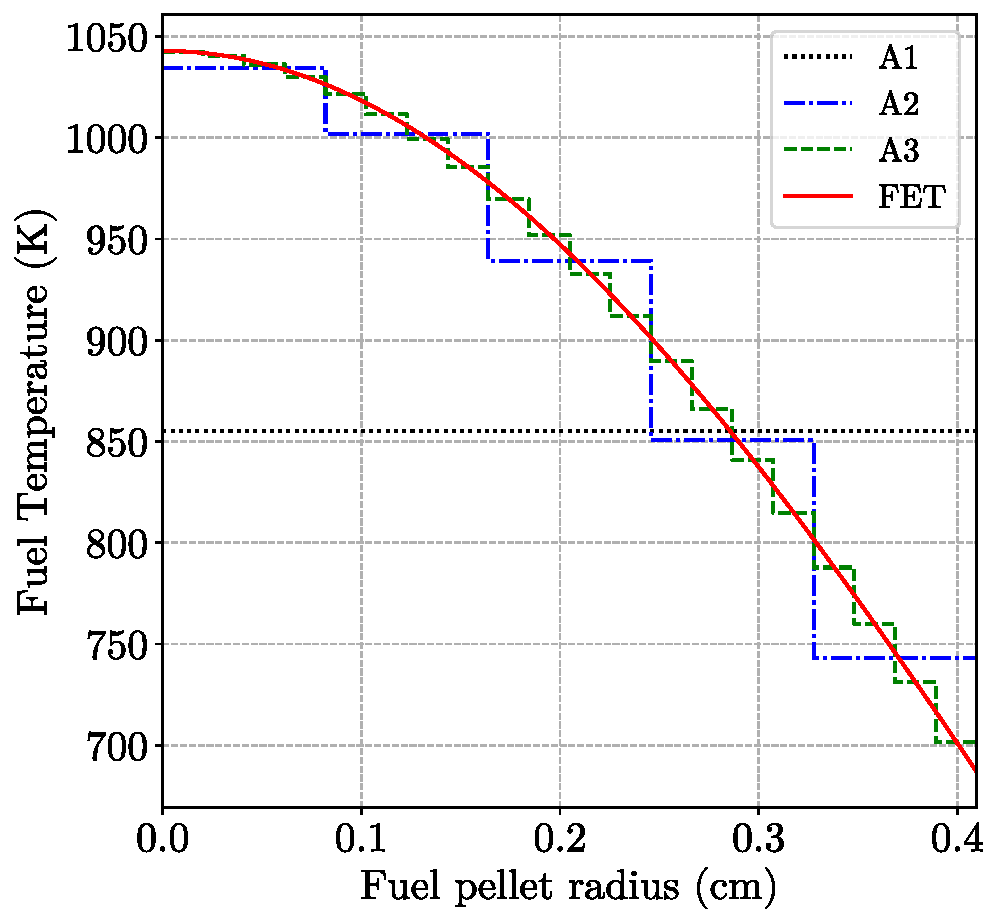
\includegraphics[width=0.5\textwidth]{figs/pin_2d_temp.pdf}
      \caption{Radial fuel temperature distribution for two-dimensional pin-cell problem.}
      \label{fig_41}
\end{figure}

\begin{figure}
    \centering
    \begin{minipage}{.49\textwidth}
      \centering
      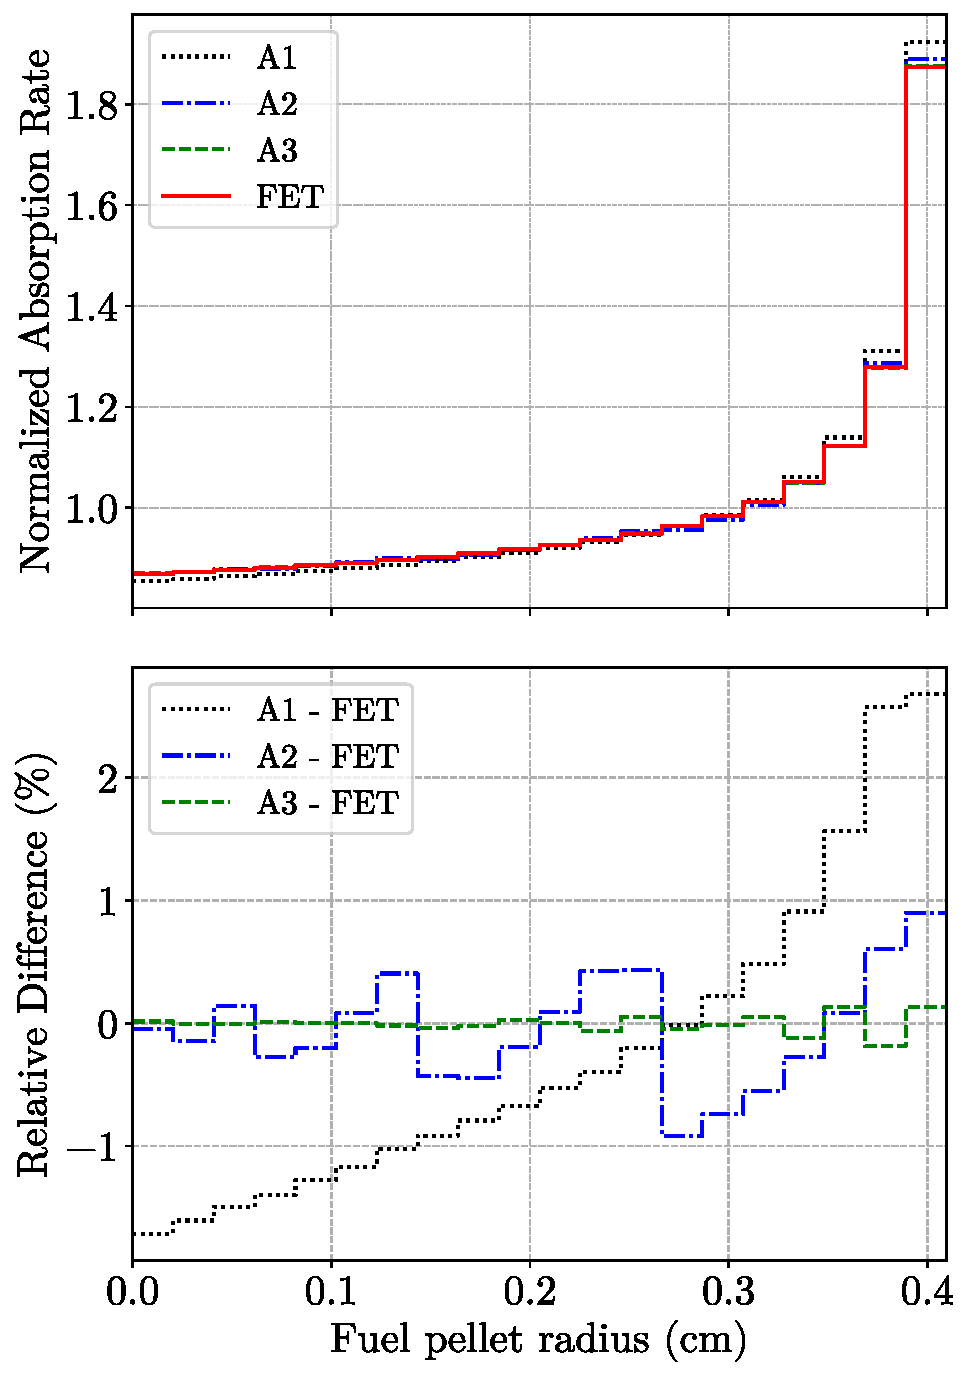
\includegraphics[width=\textwidth]{figs/pin_2d_abs.pdf}
    \end{minipage}%
    \begin{minipage}{.51\textwidth}
      \centering
      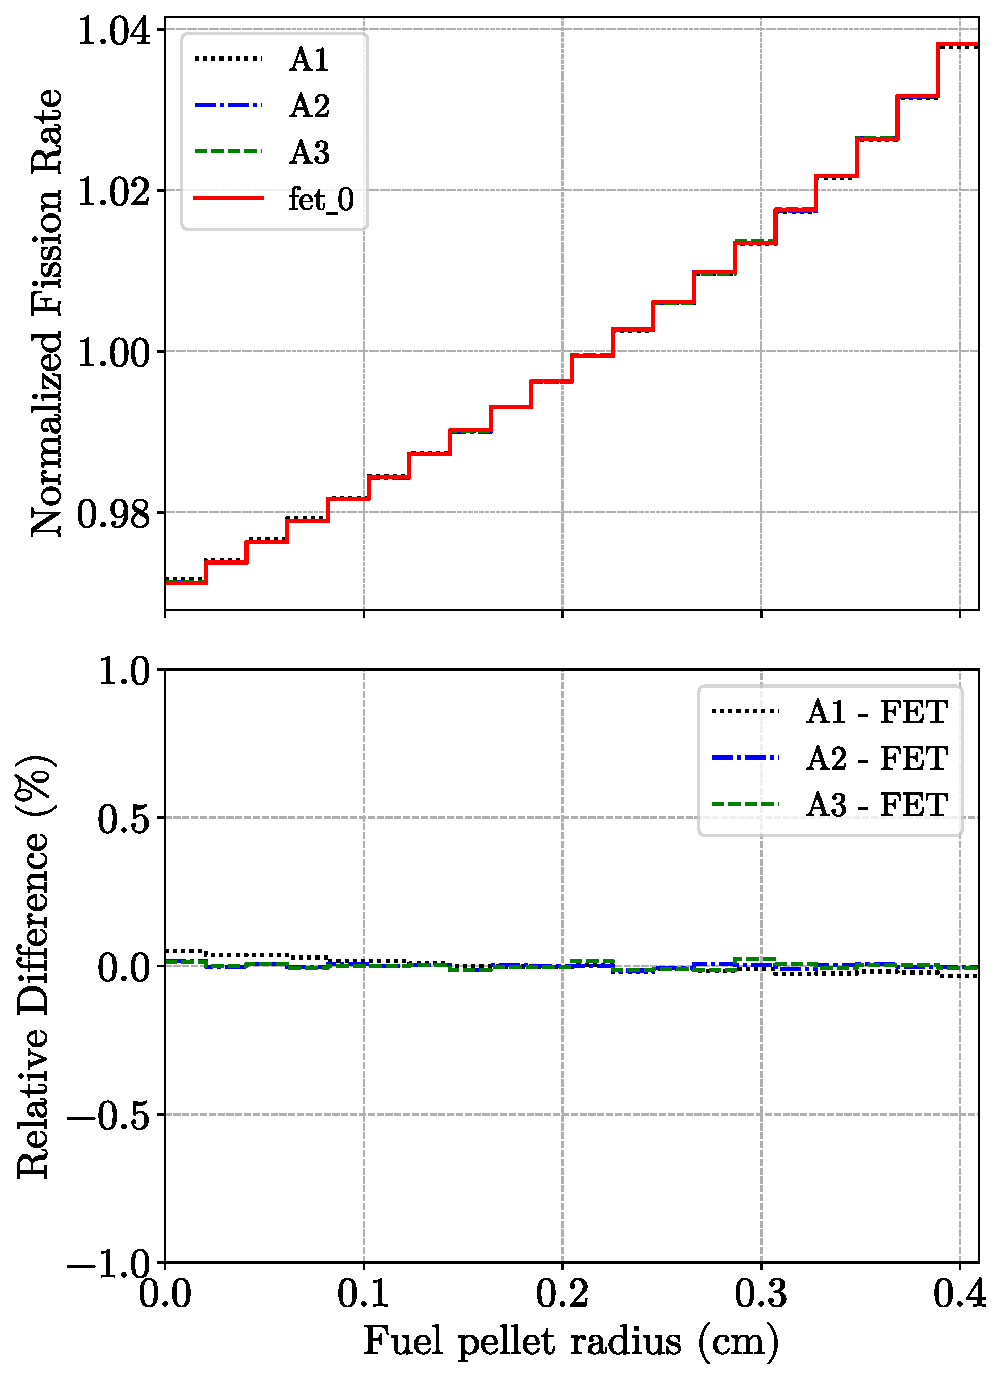
\includegraphics[width=\textwidth]{figs/pin_2d_fiss.pdf}
    \end{minipage}
    \caption[Normalized absorption and fission rates]{Normalized absorption and fission rates, and their respective relative differences for the two-dimensional pin-cell problem.}
    \label{fig_42}
\end{figure}

\begin{figure}
    \centering
    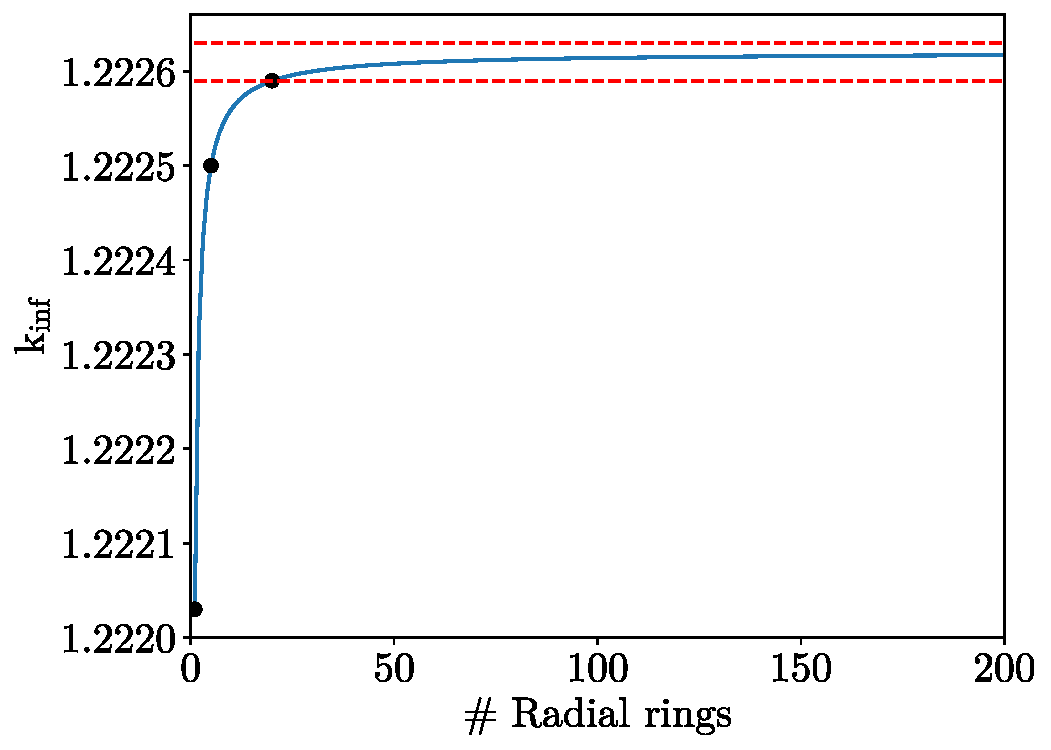
\includegraphics[width=0.6\textwidth]{figs/k_inf.pdf}
    \caption{Extrapolated $k_{inf}$ for two-dimensional pin cell problem.}
    \label{fig_43}
\end{figure}

To verify that the $k_{inf}$ from the FET case asymptotically approaches the solution obtained with infinitesimal cell sizes, a quadratic extrapolation was conducted. This extrapolation uses Lagrange basis polynomials, with the variable defined as the inverse of the number of radial rings. The extrapolated $k_{inf}$ is shown in Table \ref{tab2}, and the extrapolation result is plotted in Figure \ref{fig_43}. As illustrated, the extrapolated $k_{inf}$ lies within the uncertainty range of the $k_{inf}$ value obtained from the FET case.

These results demonstrate that the FET solutions asymptotically converge to those obtained from conventional cell-based discretized simulations with infinitesimally small cells. Furthermore, modeling radial temperature variations in the fuel pellet is essential for obtaining more accurate reactivity effects.

\subsubsection{Three-dimensional Pin-cell Problem}

This three-dimensional pin-cell problem employs UO$_2$ fuel with 2.1 wt.\% enrichment and involves two Inconel spacer grids at the top and bottom, with five Zircaloy spacer grids positioned in between. This test problem is a critical boron concentration (CBC) search problem at full power, corresponding to 67 kW of thermal power. Unlike previous problem, this problem includes equilibrium Xenon feedback.

Three cases were developed for comparison with the proposed framework. The first two cases, B1 and B2, are cell-based, where the problem domain is discretized into several cells. In the B1 case, the domain is divided into 25 axial cells and 1 radial cell, while in the B2 case, it is discretized into 100 axial cells and 5 radial cells (for the fuel pellet). The finer mesh in the B2 case is essential for capturing smoother distributions of fuel temperature, Xenon number densities (both radially and axially), and coolant density (including boron nuclide concentrations) along the axial direction. All cases simulated $5.0\times10^4$ particles per cycle over 22,500 cycles, with 20,000 active cycles.

Table \ref{tab3} compares the CBC results from all cases, showing that the solutions converge toward those obtained from the FET case as the cells' sizes become infinitesimal. This convergence is mainly due to a more accurate representation of the radial intra-fuel-pellet temperature distribution, leading to improved modeling of the self-shielding effect.
\begin{table}
    \centering
    \caption{Calculation results for three-dimensional pin-cell problem.}
    \label{tab3} 
    % \begin{adjustbox}{width=0.6\textwidth} % Adjust your table to the text width
    \begin{tabular}{| c | C{4cm} | C{3.5cm} | c | }
    \hline 
     Cases & \# of fuel pellet axial/radial discretization & Critical Boron Concentration (ppm) & Relative wall-clock time \\
     \hline
     B1     & 25/1  & $1507.5\pm0.3$ & 1.2      \\ \hline
     B2     & 100/5 & $1511.1\pm0.3$ & 4.5      \\ \hline
     FET    & N/A   & $1512.5\pm0.3$ & 1.0      \\ \hline
    \end{tabular}
    % \end{adjustbox}
\end{table}

\begin{figure}
    \centering
    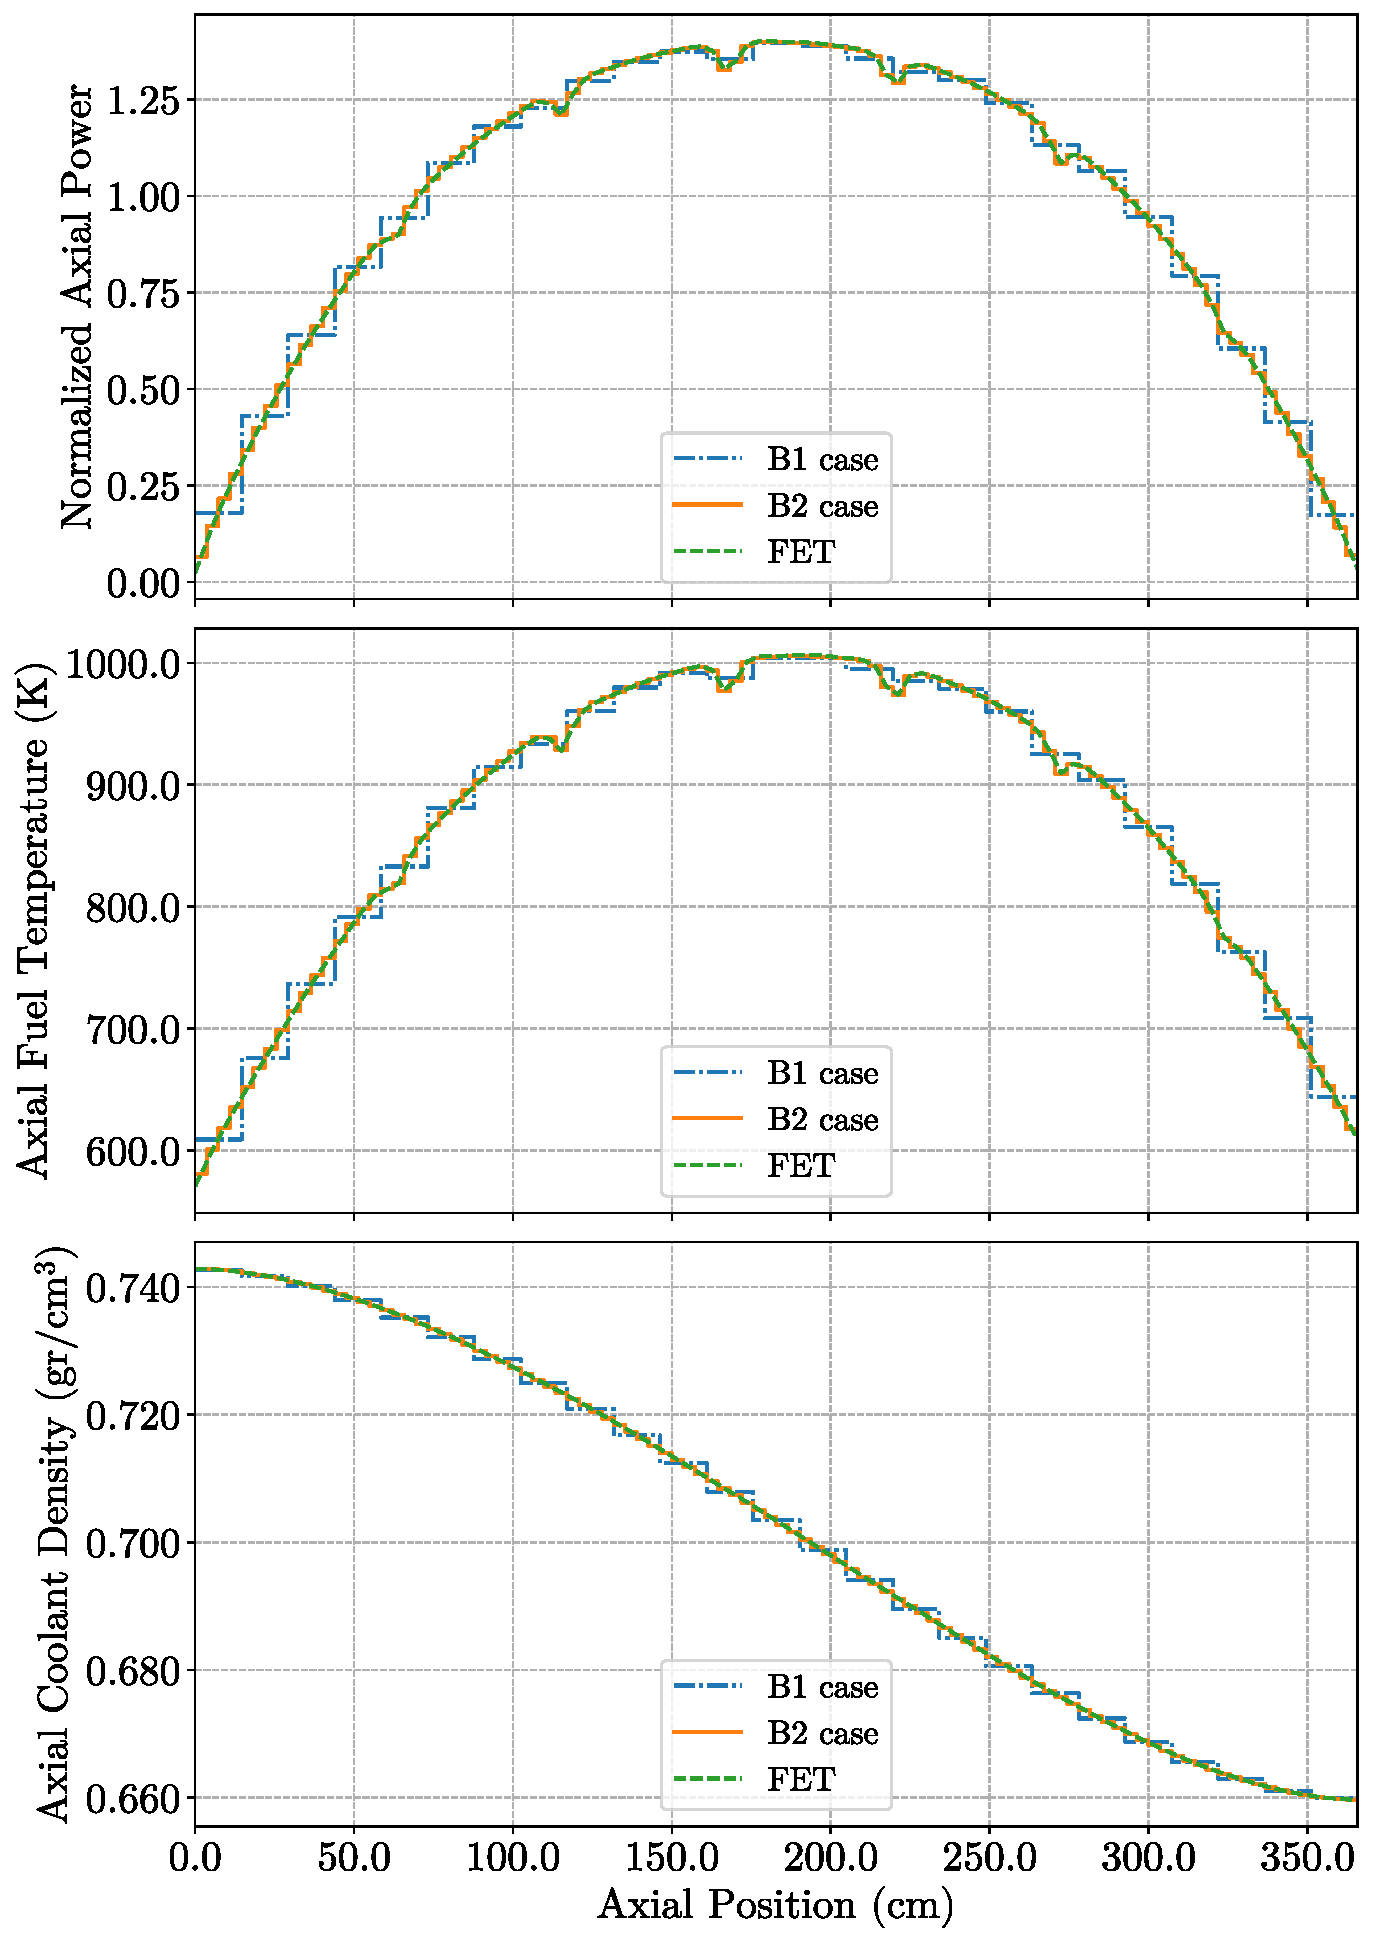
\includegraphics[width=0.75\textwidth]{figs/temp_dens.pdf}
    \caption[Normalized axial power, fuel temperature, and coolant density]{Normalized axial power, fuel temperature, and coolant density for B2 and FET cases.}
    \label{fig_44}
\end{figure}

\begin{figure}
    \centering
    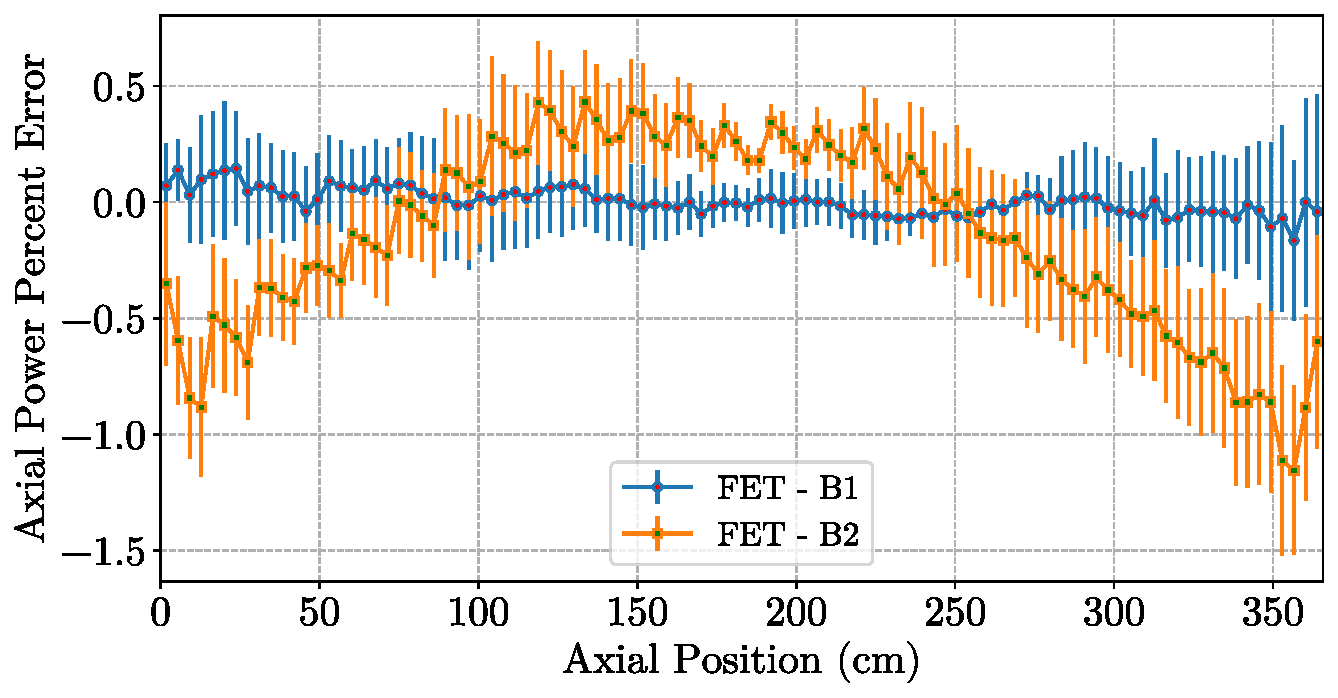
\includegraphics[width=0.75\textwidth]{figs/axial_diff.pdf}
    \caption[Axial power percentage differences of the FET case]{Axial power percentage differences of the FET case against B1 and B2 cases, and their corresponding one sigma of standard deviations.}
    \label{fig_45}
\end{figure}

Figure \ref{fig_44} illustrates the radially-averaged power, fuel temperature, and coolant density, which exhibit good agreement between cases. To further verify the accuracy of the FET case, a 100-bin axial mesh tally was performed in all cases, and percentage differences, along with one-sigma standard deviations, are presented in Figure \ref{fig_45}. As shown, the axial power differences and corresponding standard deviations between the FET and B2 cases are less than 0.5\%. These comparisons demonstrate the higher accuracy achievable with the proposed approach.

In addition, Table \ref{tab3} demonstrates that, despite its greater accuracy, the FET case has the shortest runtime. It is 1.2 and 4.5 times faster than the B1 and B2 cases, respectively. This performance improvement primarily due to reduced number of cells, which optimizes delta-tracking in two key ways. First, with fewer particle crossings, material-wise macroscopic cross-sections are computed less frequently. Second, with fewer cells, the recursive routine for determining particle location is more efficient. Moreover, in cases without localized neutron absorbers, such as burnable poisons or control rods, the rejection sampling for delta-tracking in the FET case can be performed more efficiently.

\subsubsection{Three-dimensional Assembly Problem} \label{3d_asm}

This three-dimensional assembly problem is identical to Problem \#6 from the VERA benchmark \cite{godfrey}, using 3.1 wt.\% enriched fuel pellets. This problem is simulated at hot full power (HFP), equivalent to 17.67 MW of thermal power, with 1300 ppm of boric acid diluted in the coolant. Unlike previous problem cases, this problem includes non-fuel structural materials such as the pin plenum, nozzles, core plates, and axial reflectors. Figure \ref{fig_46} illustrates the three-dimensional assembly problem.

\begin{figure}
    \centering
    \begin{minipage}{.4\textwidth}
      \centering
      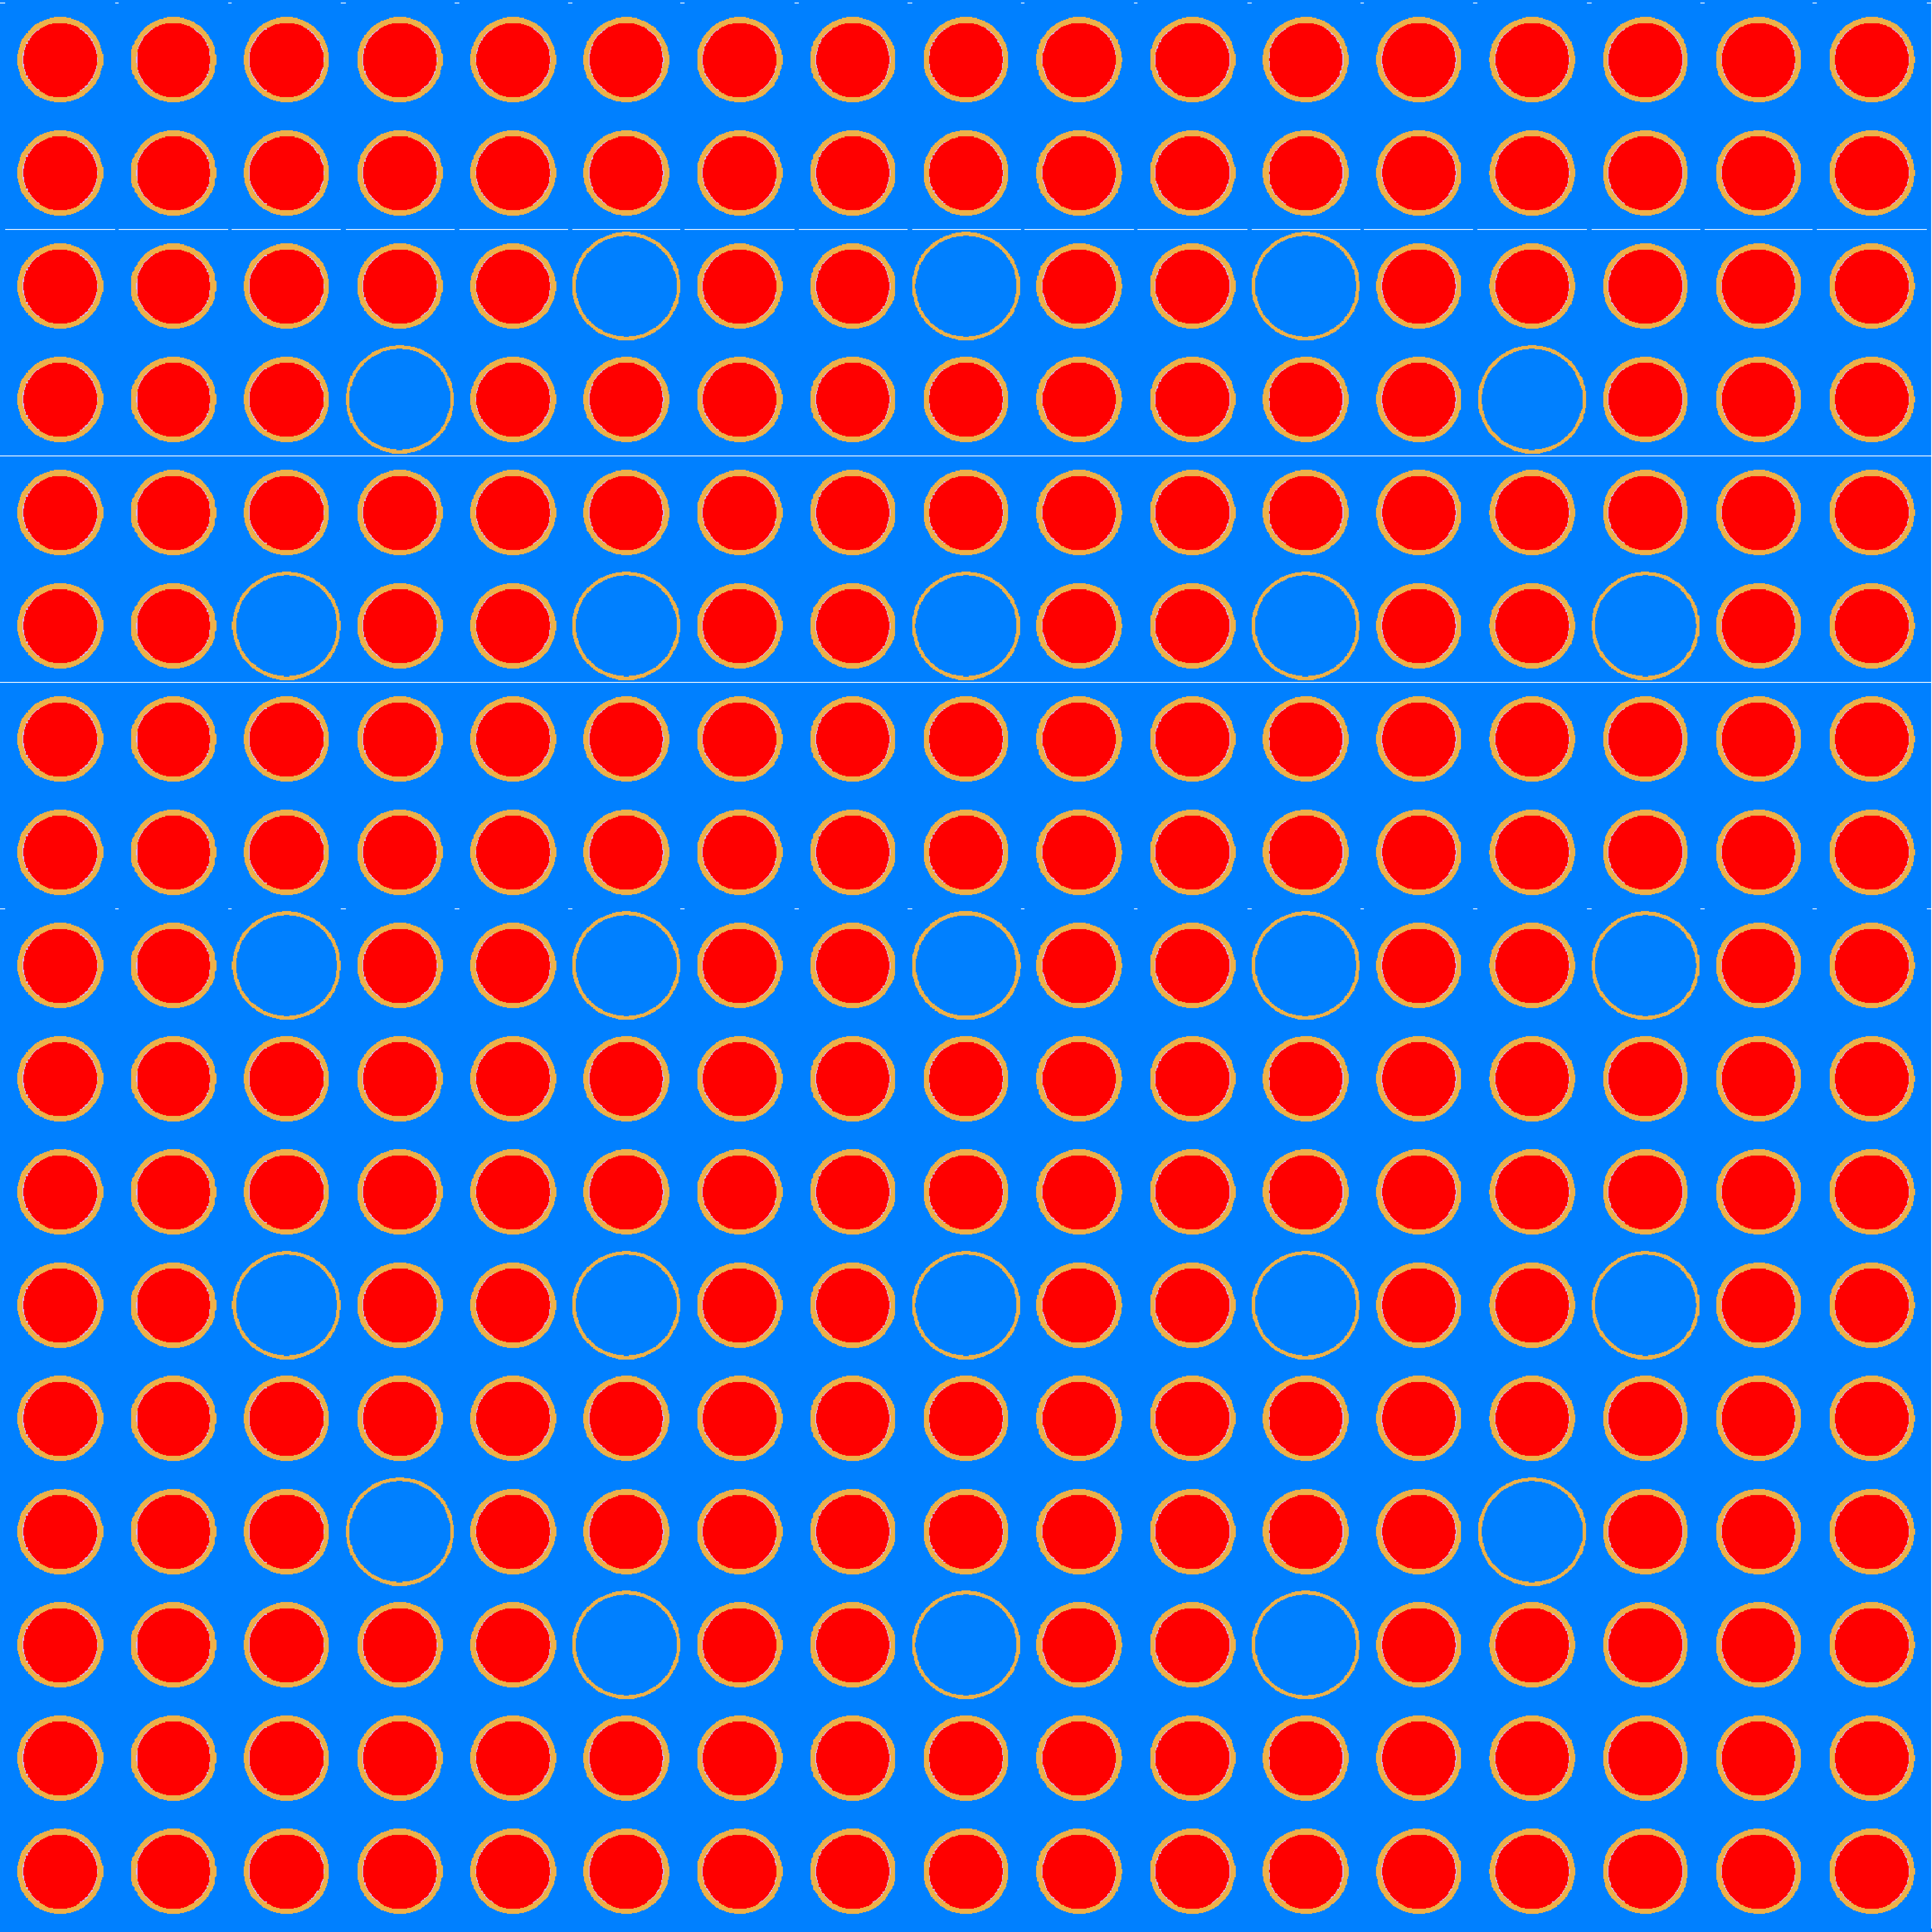
\includegraphics[width=\textwidth]{figs/radial.pdf}
    \end{minipage}%
    \hspace{10em}
    \begin{minipage}{.15\textwidth}
      \centering
      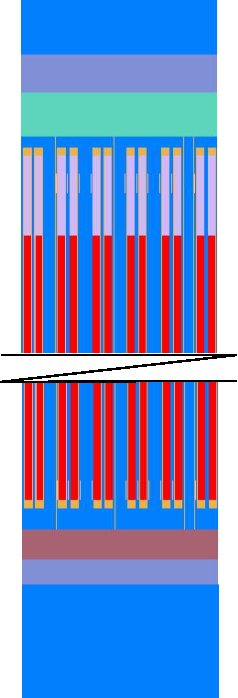
\includegraphics[width=\textwidth]{figs/axial.pdf}
    \end{minipage}
    \caption[Radial and axial geometries of the three-dimensional assembly problem]{Radial (left) and axial (right) geometries of the three-dimensional assembly problem (not to scale).}
    \label{fig_46}
\end{figure}

Four cases were developed for comparison with the proposed framework. The first three cases, C1, C2, and C3, are traditional cell-based models where the problem domain is discretized into multiple cells. In case C1, the problem is divided into 25 equidistant axial cells without radial discretization. Case C2 refines this by using 50 equidistant axial cells and 2 equivolume radial rings in the fuel pellet to capture the temperature distribution within the pellet both radially and axially. Case C3 further increases the refinement to 100 equidistant axial cells and 5 equivolume radial rings. While FET case employs spatially continuous material properties.

Each case simulated $3 \times 10^4$ particle histories per cycle, with a total of 12,500 cycles, of which 2,500 were designated as active cycles. The eigenvalue comparisons are shown in Table \ref{tab31}. As with the previous test problems, as the cell sizes become infinitesimal, the eigenvalue increases and asymptotically approaches the value from the FET case. The FET eigenvalue was also independently compared against the MC21/CTF solution \cite{kelly_2017}, with the MC21/CTF eigenvalue being approximately 40 pcm lower than the FET value.

\begin{table}
    \centering
    \caption{Calculation results for three-dimensional assembly problem.}
    \label{tab31} 
    % \begin{adjustbox}{width=0.6\textwidth} % Adjust your table to the text width
    \begin{tabular}{| c | c | c | c | }
    \hline 
     Cases & \# of fuel pellet axial/radial discretization & $k_{inf}$ & Relative wall-clock time \\
     \hline
     C1     & 25/1  & $1.16400\pm0.00004$ & 1.6      \\ \hline
     C1     & 50/2  & $1.16443\pm0.00004$ & 2.3      \\ \hline
     C2     & 100/5 & $1.16449\pm0.00005$ & 5.1      \\ \hline
     FET    & N/A   & $1.16465\pm0.00004$ & 1.0 $^\text{(a)}$      \\ \hline
    \end{tabular}
    % \end{adjustbox}
    \begin{flushleft}
        \small
        $^\text{(a)}$ The absolute wall-clock time for the FET case is 1.8 hours with 70 MPI processes. \\
    \end{flushleft}
\end{table}

\begin{figure}
    \centering
    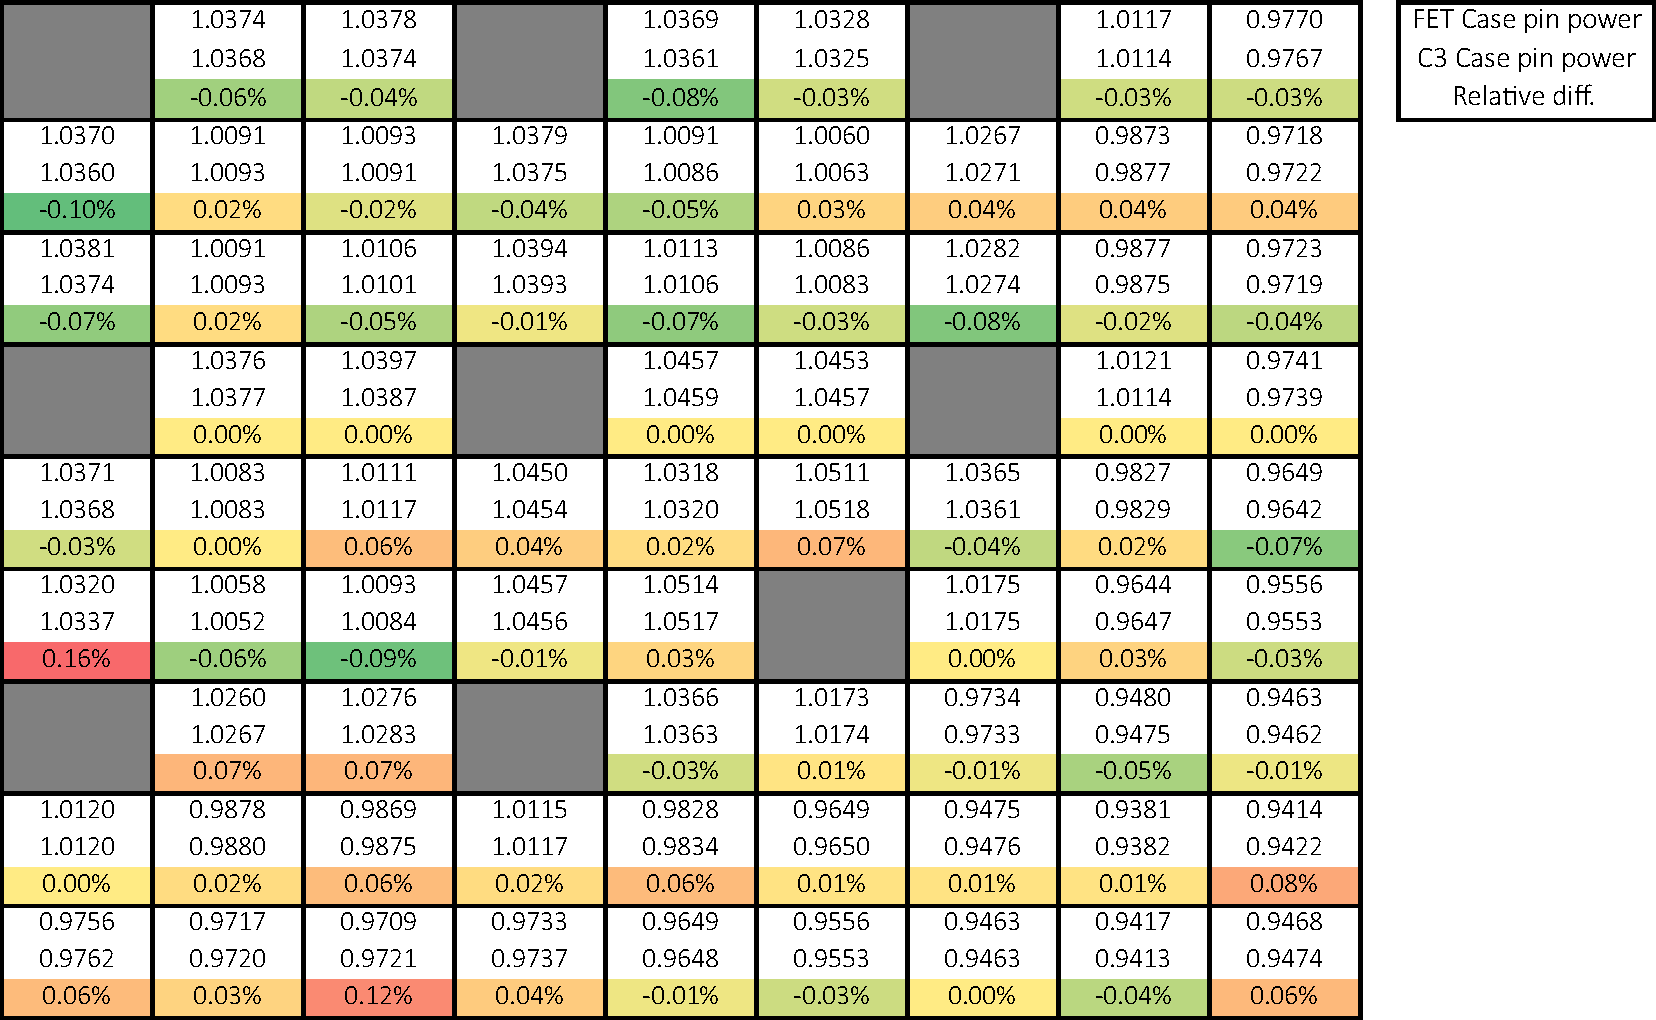
\includegraphics[width=0.95\textwidth]{figs/pin_powers.pdf}
    \caption[Pin powers comparisons for three-dimensional assembly problem.]{Pin powers from FET case are compared to case C3 for three-dimensional assembly problem.}
    \label{fig_47}
\end{figure}

The radial pin powers from the FET and C3 cases are presented in Figure \ref{fig_47}, demonstrating excellent agreement, with relative differences in pin powers being less than 0.2\% across all fuel pins. Additionally, for the assembly problem, the FET case ran 1.6, 2.3, and 5.1 times faster compared to cases C1, C2, and C3, respectively. As previously mentioned, this significant computational speedup is partly due to the absence of localized strong neutron absorbers. In the next subsection, the computational time speedup will be evaluated for assembly problems containing strong neutron absorbers.

\subsubsection{Three-dimensional Assembly Problem with Neutron Absorbers}

This test problem aims to evaluate the computational time speedup of the FET case for reactor problems with strong neutron absorbers. The presence of neutron absorbers is expected to reduce the efficiency of the rejection sampling in the delta-tracking method. The problem setup is identical to the assembly problem described in subsection \ref{3d_asm}, with the exception that either Pyrex or control rods are inserted into the guide tubes.

As previously described, the tip of the control rod is made from AIC, measuring 101.6 cm in length, while the remaining 259.05 cm is composed of boron carbide. In this problem, the control rod is inserted to a depth of 186 steps (where 1 step corresponds to 1.5875 cm), meaning only the AIC portion is inserted into the active core. This configuration makes the presence of the neutron absorber more localized, while the Pyrex burnable poisons occupy almost the entire active core axially.

Table \ref{tab32} provides $k_{inf}$ solutions along with relative simulation times. As can be observed, the presence of Pyrex has little effect on the FET case speedup compared to problems without Pyrex, as shown in Table \ref{tab31}. This is because the presence of Pyrex is not localized, so the rejection sampling procedure in the delta-tracking can still be performed efficiently.

In contrast, the presence of control rods is very localized, located in a small portion at the top of the active core. This leads to poor rejection sampling efficiency in the delta-tracking method. As seen in Table \ref{tab32}, the FET speedup compared to a 100/5 axial/radial discretization with control rods inserted at 186 steps is 2.6 times. This speedup is much smaller than for problems without the control rods inserted, which is around 5.1 times, as observed in Table \ref{tab31}. The $k_{inf}$ solutions generally follow the same trend as in previous problems, where they converge to the FET case solutions for infinitesimal cells.

\begin{table}
    \centering
    \caption[Calculation results for assembly problem with neutron absorbers.]{Calculation results for three-dimensional assembly problem with neutron absorbers.}
    \label{tab32} 
    % \begin{adjustbox}{width=\textwidth} % Adjust your table to the text width
    \begin{tabular}{| c | C{0.16\linewidth} | c | C{0.12\linewidth} | c | C{0.12\linewidth} | }
    \hline 
           &        &  \multicolumn{2}{c|}{Pyrex} & \multicolumn{2}{c|}{Control Rods}  \\
    \cline{3-6}
    Cases & \# of fuel pellet axial/radial discretization & $k_{inf}$ & Relative wall-clock time & $k_{inf}$ & Relative wall-clock time \\
    \hline
    D1     & 25/1  & $0.95876\pm0.00004$ & 1.5  & $1.15972\pm0.00004$ & 0.8     \\ \hline
    D1     & 50/2  & $0.95909\pm0.00004$ & 2.1  & $1.16007\pm0.00004$ & 1.1     \\ \hline
    D2     & 100/5 & $0.95918\pm0.00004$ & 4.7  & $1.16027\pm0.00004$ & 2.6     \\ \hline
    FET    & N/A   & $0.95929\pm0.00004$ & 1.0 $^\text{(a)}$  & $1.16047\pm0.00004$ & 1.0 $^\text{(b)}$      \\ \hline
    \end{tabular}
    % \end{adjustbox}
    \begin{flushleft}
        \small
        $^\text{(a)}$ The absolute wall-clock time for the FET case is 1.9 hours with 70 MPI processes. \\
        $^\text{(b)}$ The absolute wall-clock time for the FET case is 3.5 hours with 70 MPI processes. \\
    \end{flushleft}
\end{table}


\subsubsection{Whole-core Reactor Problem} \label{wc}

The final test problem for the spatially continuous material properties is a whole-core problem, based on Problem \#7 of the VERA benchmark: a three-dimensional, beginning-of-cycle (BOC) physical reactor. This benchmark provides detailed descriptions of the reactor core geometry and internal structures. Figure \ref{fig_4a} illustrates the detailed whole-core reactor geometry modeling of the VERA benchmark in MCS. This test problem estimates the CBC at HFP.

\begin{figure}
    \centering
    \begin{subfigure}[b]{0.55\textwidth}
        \centering
        \includegraphics[width=\textwidth]{figs/xy_wb.pdf}
        \caption{Radial view.}
    \end{subfigure}
    \hspace{10em}
    \begin{subfigure}[b]{0.36\textwidth}
        \centering
        \includegraphics[width=\textwidth]{figs/xz_wb.pdf}
        \caption{Axial view.}
    \end{subfigure}
    \caption{Detailed whole-core reactor geometry modelling in MCS.}
       \label{fig_4a}
\end{figure}

As with the previous test problems, several cases were developed to compare the spatially continuous material approach with the cell-based approach. These cases, along with descriptions of the cell discretizations, are listed in Table \ref{tab33}. Note that all simulations utilized \(6 \times 10^4\) particles per cycle, over a total of 37,500 cycles, with 30,000 cycles designated as active. This number of particle of histories produces axially averaged pin-power densities with maximum standard deviation around 0.6\%. In this problem, the reactor is modelled in a quarter core.

In the MCS modeling for the FET case, each fuel assembly has different delta-tracking region, with each assembly having its own majorant cross-section. Therefore, when a particle crosses an assembly surface, the particle track must be terminated. Subsequently, a new sampling of the distance to collision must be calculated using a different majorant cross-section. Additionally, the withdrawn RCCAs are excluded from the delta-tracking region to optimize the rejection sampling procedure. c Therefore, to improve performance, the withdrawn RCCAs are not included in the delta-tracking region in the FET case.

The CBC results are presented in Table \ref{tab33}. As shown in the table, the behavior of the solutions is similar to those from the previous problems, where the CBC from the cell-based converges to that from the FET case using spatially continuous material properties. The CBC difference, compared to the E1 case with 25/1 radial/axial cell discretizations, is around 7 ppm, corresponding to approximately 70 pcm of reactivity. This result is consistent with previous solutions. Moreover, the FET case only requires one-third of the simulation time to achieve similar or even better accuracy compared to the E2 case with 60/5 radial/axial cell discretizations.

In this whole-core problem, the random access memory (RAM) requirements were also evaluated. The memory usage was measured in the Ubuntu operating system using the \code{free -m} command during the simulation. As shown in the table, the FET case requires only 20\% of the RAM compared to the E3 case. This reduction in memory usage is mainly due to the fewer number of cells employed in the FET case. Although there is additional memory needed to store the FET coefficients, the number of coefficients is too small to offset the overall memory reduction. This demonstrates that the use of spatially continuous materials with FET not only achieves better accuracy with less simulation time, but also requires lower memory usage.

\begin{table}
    \centering
    \caption{Calculation results for whole-core problem.}
    \label{tab33} 
    % \begin{adjustbox}{width=\textwidth} % Adjust your table to the text width
        \begin{tabular}{| c | C{0.25\linewidth} | c | C{0.2\linewidth} | C{0.2\linewidth} | }
            \hline 
            Cases & \# of fuel pellet axial/radial discretization & CBC (ppm) & Relative wall-clock time & Relative memory usage \\
            \hline
            E1     & 25/1  & $859.6\pm0.2$ & 1.2 & 1.1      \\ \hline
            E1     & 50/2  & $863.0\pm0.2$ & 1.8 & 2.4      \\ \hline
            E2     & 60/5  & $864.0\pm0.2$ & 2.9 & 4.9      \\ \hline
            FET    & N/A   & $866.2\pm0.2$ & 1.0 $^\text{(a)}$ & 1.0 $^\text{(b)}$      \\ \hline
        \end{tabular}
    % \end{adjustbox}
    \begin{flushleft}
        \small
        $^\text{(a)}$ The absolute wall-clock time for the FET case is 14.3 hours with 70 MPI processes. \\
        $^\text{(b)}$ The absolute memory usage for the FET case is 146.4 GB per node, with each node running 35 MPI processes.
    \end{flushleft}
\end{table}

Figure \ref{fig_49} shows the assembly power map and its comparison between the FET and E3 cases. As observed, the maximum and minimum assembly power relative differences are approximately 0.3\%, with a root mean squared error (RMS) of 0.2\%. And the relative difference on axial power, shown in Figure \ref{fig_49a}, is also less than 1\%. At the pin level, the normalized radial pin-power densities also exhibit good agreement between the FET and E3 cases, with an RMS of 0.3\%, and maximum and minimum relative differences of less than 2\%, as shown in Figure \ref{fig_48}. Additionally, the three-dimensional view of radially pin-averaged coolant and  fuel temperatures from FET case are plotted in Figure \ref{fig_49b}. These results confirm that the solutions with spatially continuous material properties are well aligned with the cell-based cases that use very small cells.

\begin{figure}
    \centering
    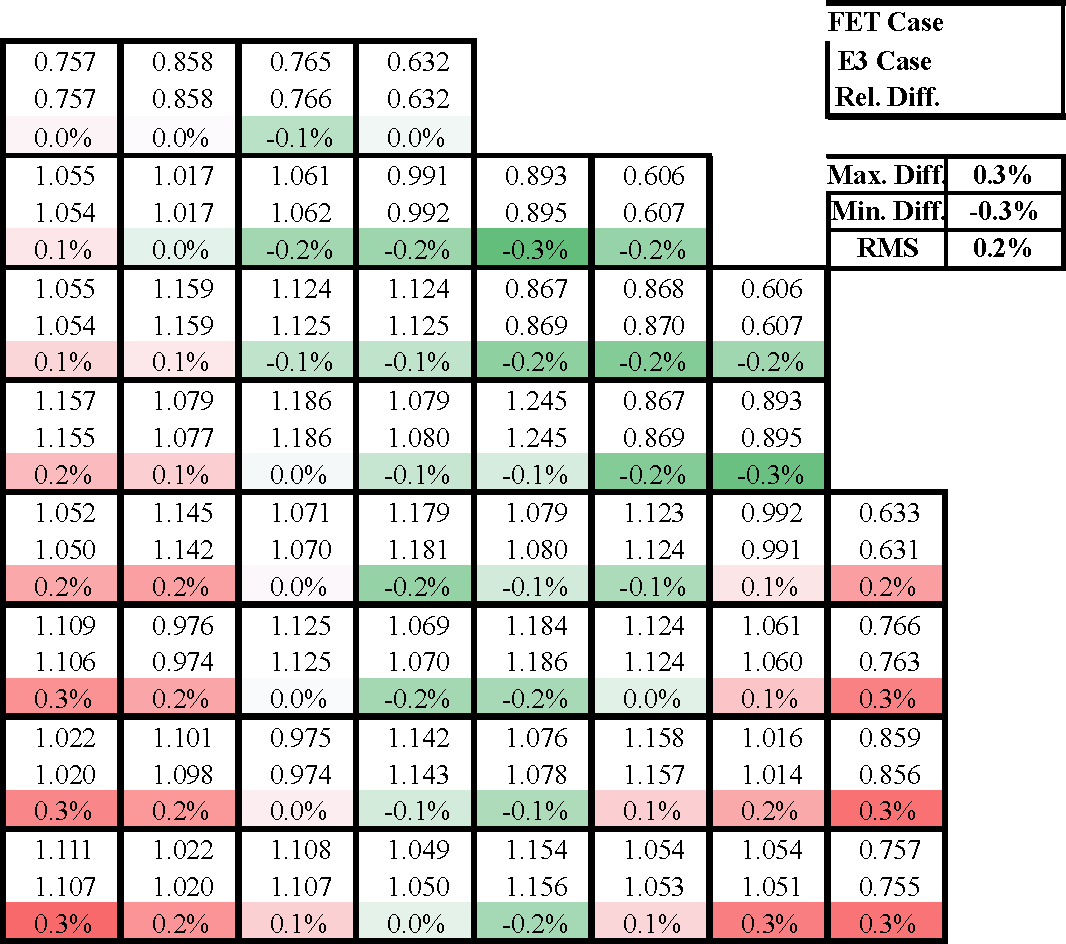
\includegraphics[width=0.8\textwidth]{figs/asm_power.pdf}
    \caption{Assembly powers comparison between FET and E3 cases.}
    \label{fig_49}
\end{figure}

\begin{figure}
    \centering
    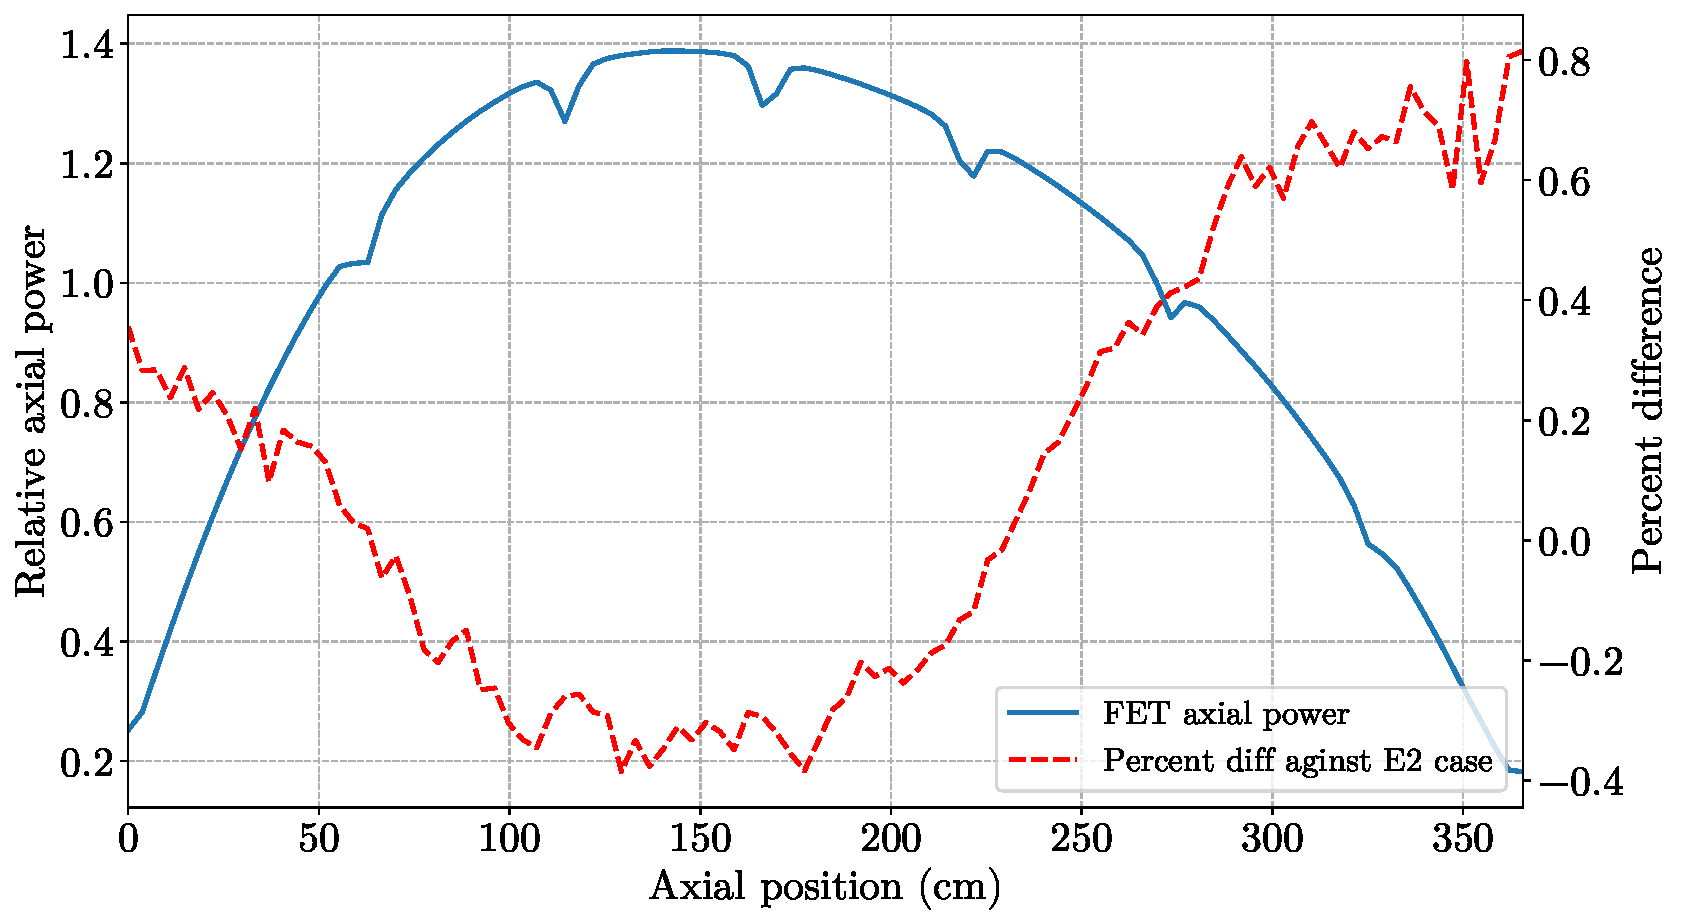
\includegraphics[width=0.9\textwidth]{figs/axial_pow.pdf}
    \caption[Axial power comparison for the whole-core problem.]{Axial power from FET case compared with that from E3 case for the whole-core problem.}
    \label{fig_49a}
\end{figure}

\begin{figure}
    \centering
    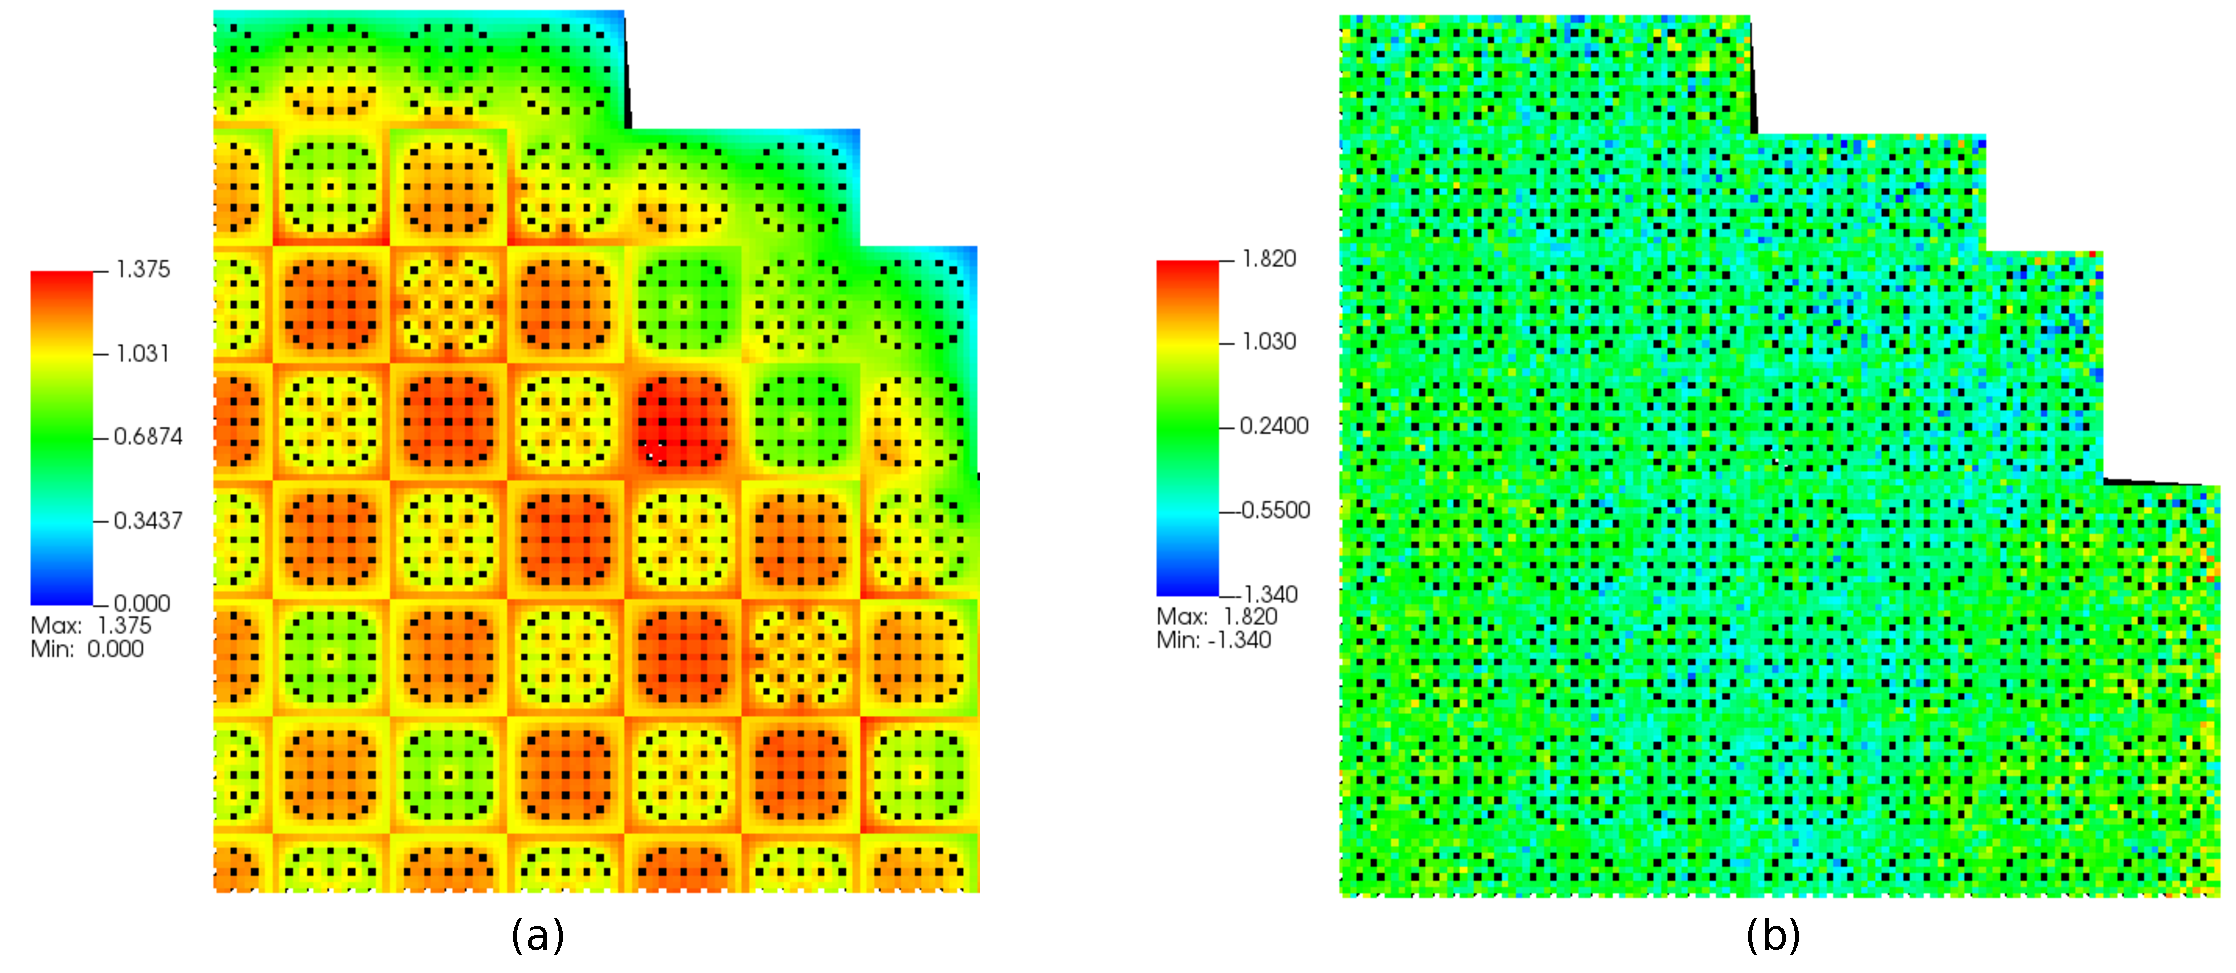
\includegraphics[width=1.0\textwidth]{figs/core_fet.pdf}
    \caption[Normalized radial pin-power densities of the FET case for the whole-core problems]{Normalized radial pin-power densities of the FET case for the whole-core problems (a), and their comparisons against E3 case (b).}
    \label{fig_48}
\end{figure}

\begin{figure}
    \centering
    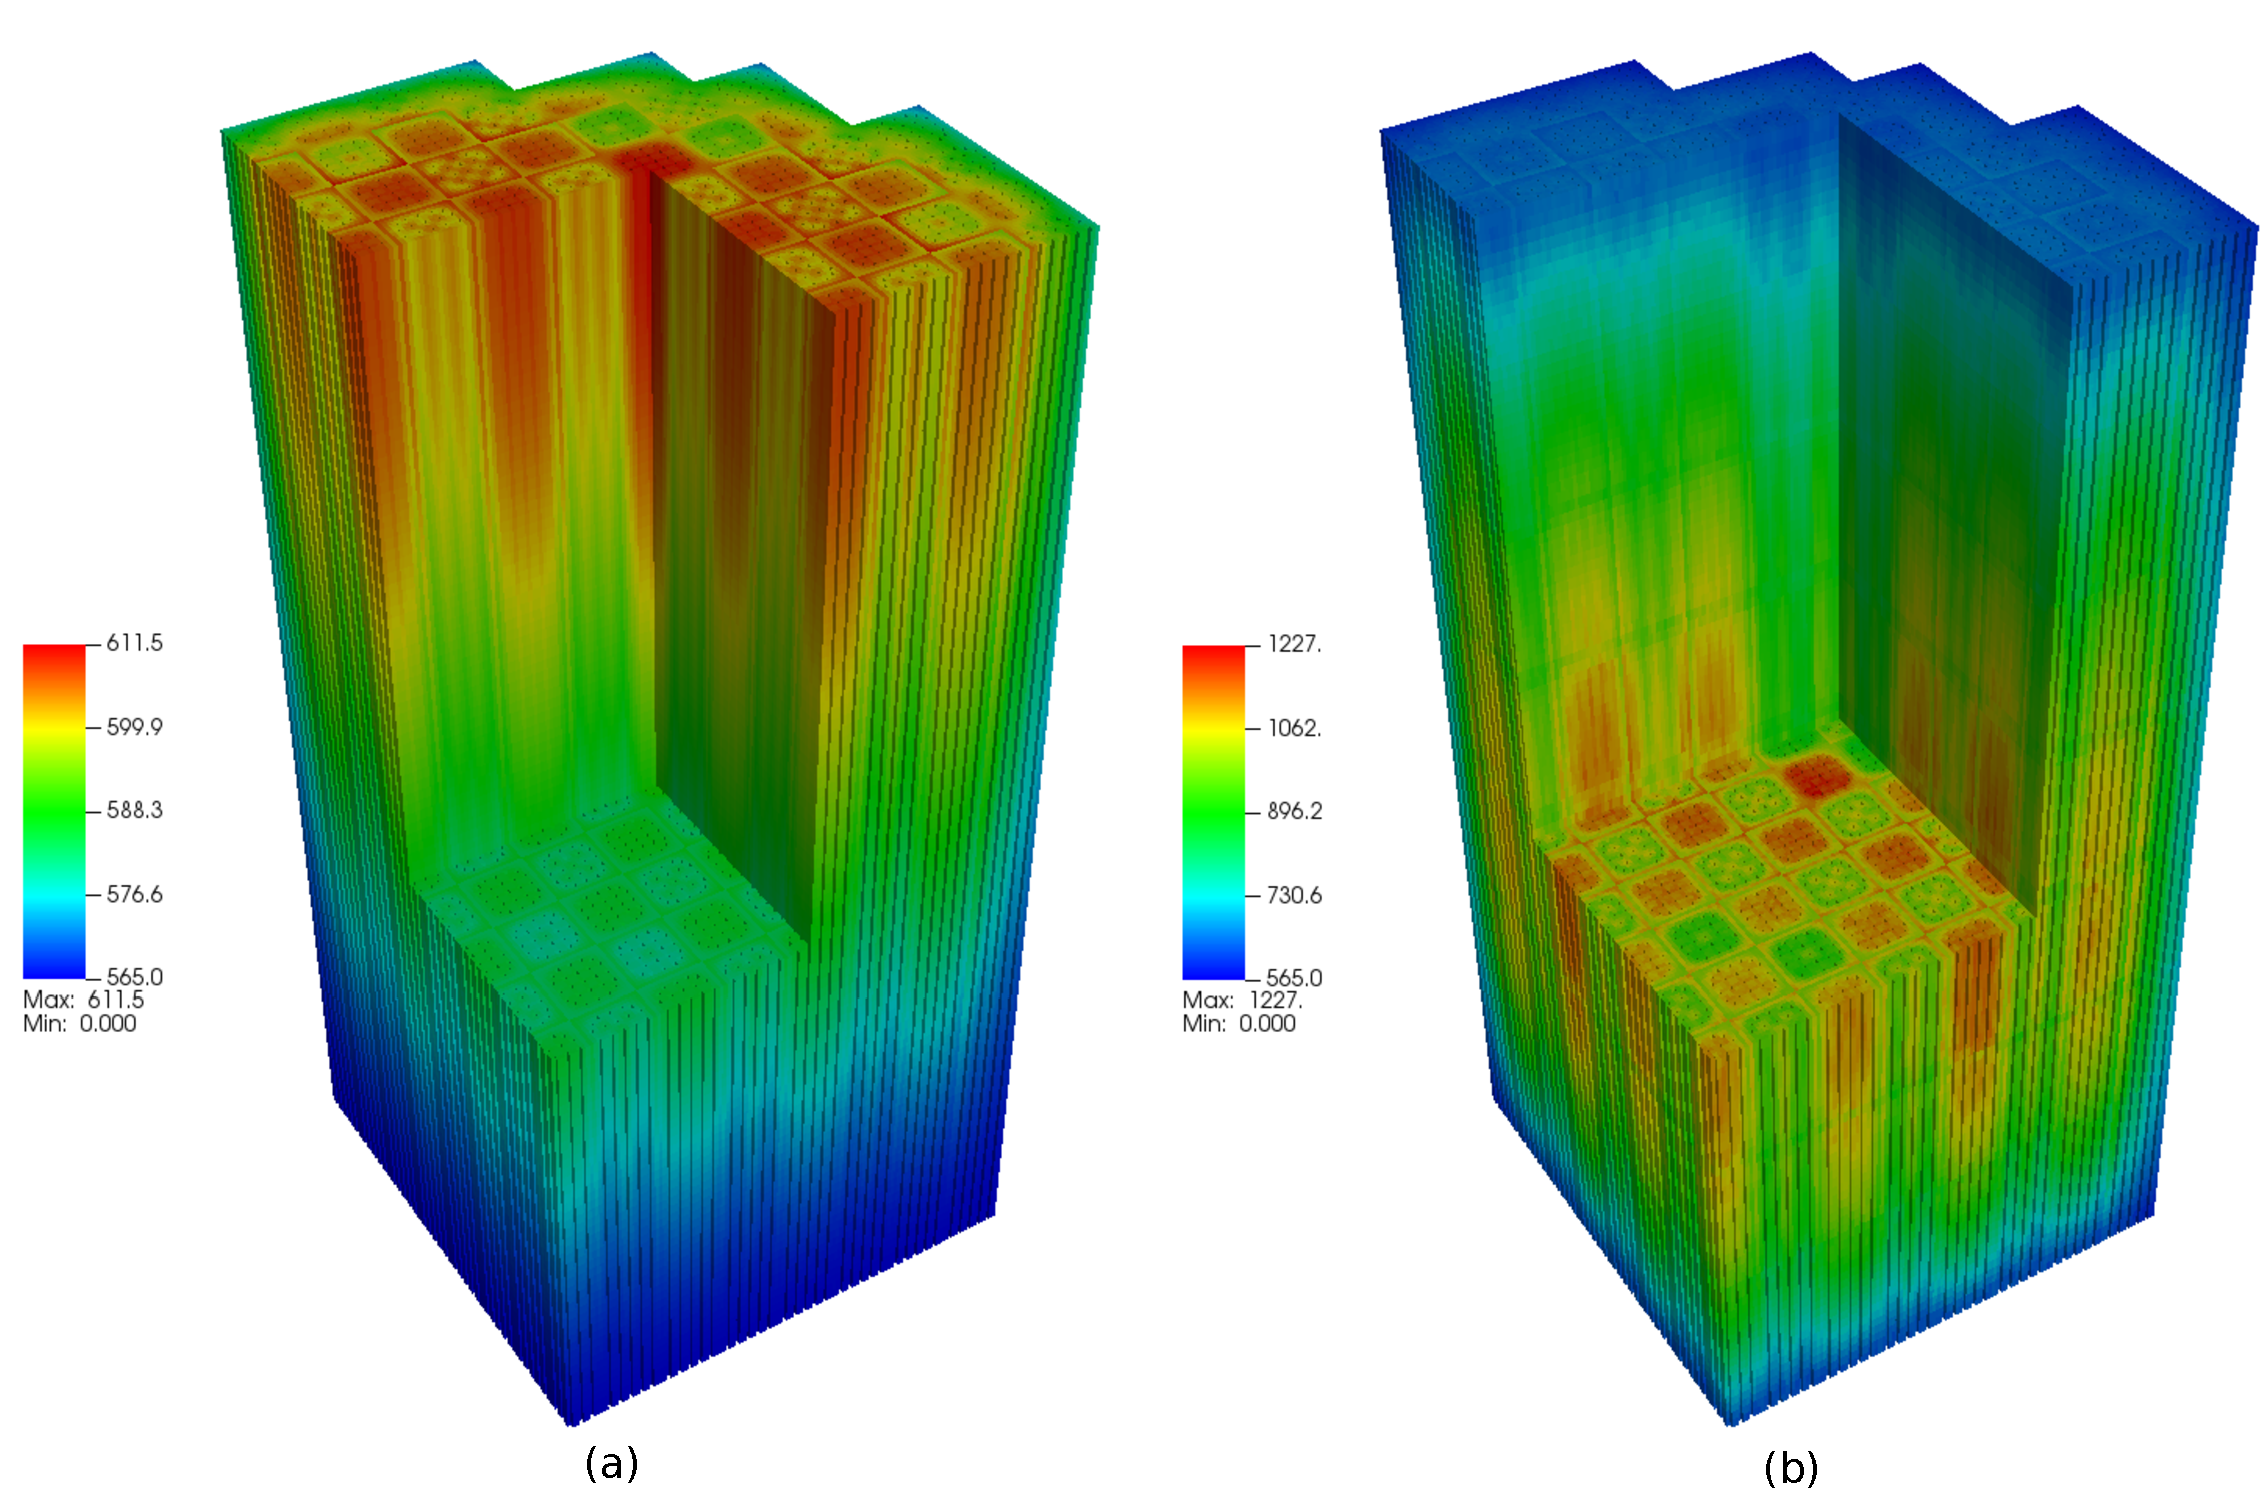
\includegraphics[width=1.0\textwidth]{figs/fuel.pdf}
    \caption[Three-dimensional view of radially pin-averaged coolant and  fuel temperatures]{Three-dimensional view of radially pin-averaged coolant temperature (a) and fuel temperature (b) from FET case.}
    \label{fig_49b}
\end{figure}

A set of FET cases utilizing various orders of Zernike and Legendre polynomials was conducted to assess the effects of polynomial order on accuracy, running time, and memory usage. The results for these cases are presented in Table \ref{tab34}. It should be noted that in Table \ref{tab34}, the Zernike and Legendre polynomials are of the same order for each case. Additionally, the running time and memory usage are calculated relative to the $8^\text{th}$ order case.

\begin{table}
    \centering
    \caption{Calculation results for FET cases utilizing different orders of Zernike and Legendre polynomials.}
    \label{tab34} 
    % \begin{adjustbox}{width=\textwidth} % Adjust your table to the text width
        \begin{tabular}{| c | c | C{0.2\linewidth} | C{0.2\linewidth} | }
            \hline 
            Zernike and Legendre order &  CBC (ppm) & Relative wall-clock time & Relative memory usage \\
            \hline
            $2^\text{nd}$   & $866.0\pm0.2$ & 0.90 & 0.70      \\ \hline
            $4^\text{th}$   & $866.1\pm0.2$ & 0.93 & 0.80      \\ \hline
            $6^\text{th}$   & $865.7\pm0.2$ & 0.97 & 0.90      \\ \hline
            $8^\text{th}$   & $865.6\pm0.2$ & 1.00 $^\text{(a)}$ & 1.00 $^\text{(b)}$      \\ \hline
            $10^\text{th}$  & $866.0\pm0.2$ & 1.03 & 1.10      \\ \hline
        \end{tabular}
    % \end{adjustbox}
    \begin{flushleft}
        \small
        $^\text{(a)}$ The absolute wall-clock time for the $8^\text{th}$ order case is 14.5 hours with 70 MPI processes. \\
        $^\text{(b)}$ The absolute memory usage for the $8^\text{th}$ order case is 153.1 GB per node, with each node running 35 MPI processes.
    \end{flushleft}
\end{table}

As can be seen in Table \ref{tab34}, the solution accuracy for CBC is quite good even with the use of $2^\text{nd}$ order Zernike and Legendre polynomials. The results for these $2^\text{nd}$ order polynomials still fall within the statistical uncertainties for both CBC and power distribution, making it difficult to compare their accuracy. However, the use of low-order polynomials is generally not recommended for broader problems, as it may compromise calculation accuracy. Interesting observations can be made regarding how the polynomial order impacts running time and memory usage: an increase in polynomial order by two leads to a 3\% increase in running time. Similarly, an increase in two polynomial order results in approximately a 10\% rise in memory usage. Thus, it is evident that the polynomial order significantly affects memory usage during MC multi-physics coupled simulations that utilize spatially continuous material properties.